\documentclass[12pt]{article}
 \usepackage[margin=1in]{geometry} 
\usepackage{amsmath,amsthm,amssymb,amsfonts, pgfplots}
\usepackage{stackengine}
 
 \newcommand{\longdiv}[2]{$#1\overline{\smash{)}#2}$}
\newcommand{\N}{\mathbb{N}}
\newcommand{\Z}{\mathbb{Z}}
 
\newenvironment{problem}[2][Problem]{\begin{trivlist}
\item[\hskip \labelsep {\bfseries #1}\hskip \labelsep {\bfseries #2.}]}{\end{trivlist}}
 
 
 
\begin{document}
\title{Experimenting with Plots}
\author{Mia Jones}

\maketitle


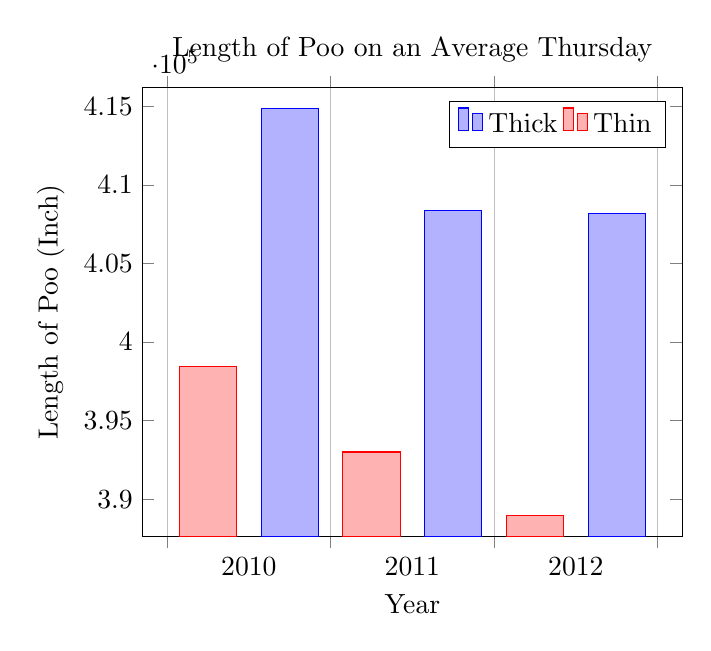
\begin{tikzpicture}
\begin{axis}[
	x tick label style={
		/pgf/number format/1000 sep=},
	title=Length of Poo on an Average Thursday,
	xlabel=Year,
	ylabel=Length of Poo (Inch),
	enlargelimits=0.05,
	legend style={at={(0.5,-0.1)},
	anchor=north,legend columns=-1},
	ybar interval=0.7,
	legend pos= north east,
]

\addplot 
	coordinates {(2012,408184) (2011,408348)
		 (2010,414870) (2009,412156)};
\addplot 
	coordinates {(2012,388950) (2011,393007) 
		(2010,398449) (2009,395972)};
\legend{Thick, Thin}
\end{axis}
\end{tikzpicture}

\end{document}